% This text is proprietary.
% It's a part of presentation made by myself.
% It may not used commercial.
% The noncommercial use such as private and study is free
% Dec 2007
% Author: Sascha Frank
% University Freiburg
% www.informatik.uni-freiburg.de/~frank/
%
%
\documentclass{beamer}
\setbeamertemplate{navigation symbols}{}


\usetheme{Montpellier}

\usepackage{tikz}

\beamersetuncovermixins{\opaqueness<1>{25}}{\opaqueness<2->{15}}
\begin{document}
\title{\TeX / \LaTeX \, Class WCC}
\author{Antje Kazimiers}
\date{\today}
\begin{frame}
\titlepage
\end{frame}

\begin{frame}\frametitle{Table of contents}
    \tableofcontents
\end{frame}


\section{Introduction}
\subsection{What is TeX / What is \LaTeX}
\begin{frame}
    \frametitle{What is TeX / What is LaTex}
\end{frame}

\begin{frame}
    \frametitle{Not WYSIWYG!}
    What you see is what you get
\end{frame}


\subsection{Examples}
\begin{frame}\frametitle{unnumbered lists}
\begin{itemize}
    \item Introduction to  \LaTeX
    \item Course 2
    \item Termpapers and presentations with \LaTeX
    \item Beamer class
\end{itemize}
\end{frame}

\begin{frame}\frametitle{lists with pause}
\begin{itemize}
    \item Introduction to  \LaTeX \pause
    \item Course 2 \pause
    \item Termpapers and presentations with \LaTeX \pause
    \item Beamer class
\end{itemize}
\end{frame}

\subsection{Math}
\begin{frame}\frametitle{Math equations}
%https://www.overleaf.com/learn/latex/Mathematical_expressions#Mathematical_modes
$$\int_{a}^{b} x^2 dx $$

\[\left(  \frac{ N } { \left( \frac{L}{p} \right)  - (m+n) }  \right]   \]
\end{frame}

\begin{frame}\frametitle{numbered lists with pause}
\begin{enumerate}
    \item Introduction to  \LaTeX \pause
    \item Course 2 \pause
    \item Termpapers and presentations with \LaTeX \pause
    \item Beamer class
\end{enumerate}
\end{frame}

\section{Pictures}
\subsection{Tables}
\begin{frame}\frametitle{Tikz}
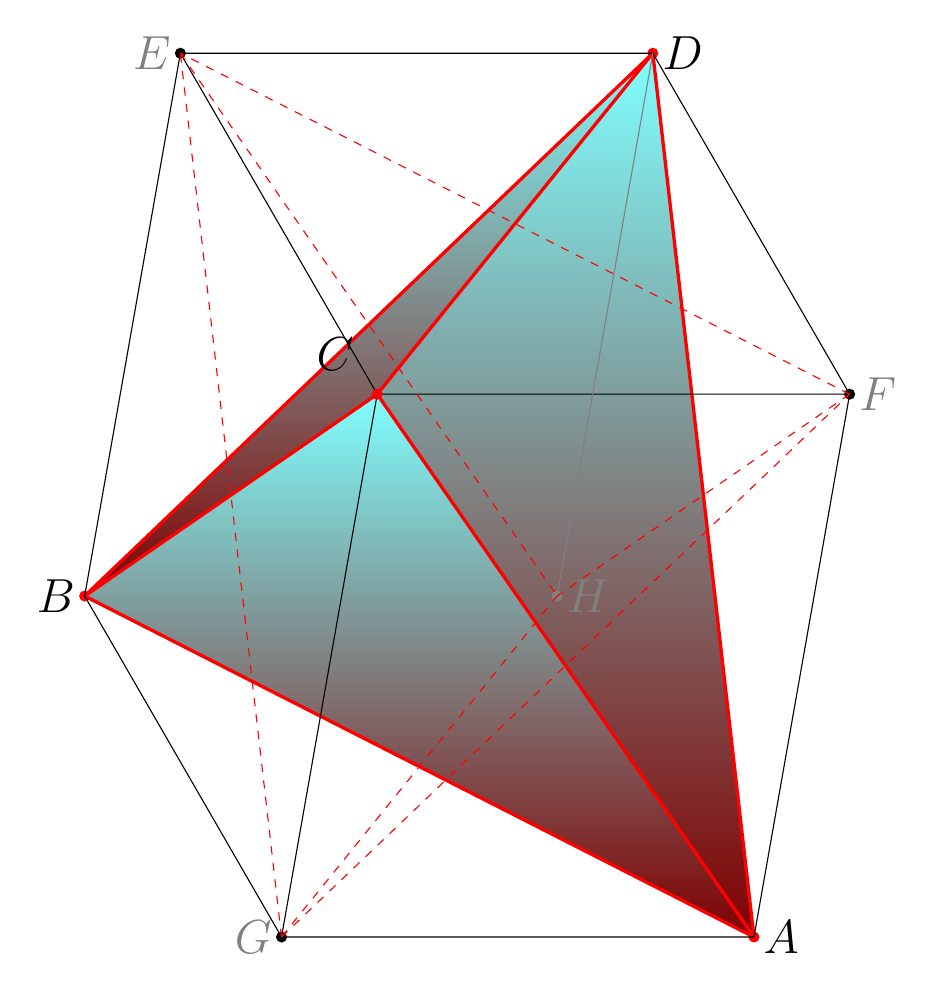
\begin{tikzpicture}[font=\LARGE]

% Figure parameters (tta and k needs to have the same sign)
% They can be modified at will
\def \tta{ -10.00000000000000 } % Defines the first angle of perspective
\def \k{    -3.00000000000000 } % Factor for second angle of perspective
\def \l{     6.00000000000000 } % Defines the width  of the parallelepiped
\def \d{     5.00000000000000 } % Defines the depth  of the parallelepiped
\def \h{     7.00000000000000 } % Defines the heigth of the parallelepiped

% The vertices A,B,C,D define the reference plan (vertical)
\coordinate (A) at (0,0);
\coordinate (B) at ({-\h*sin(\tta)},{\h*cos(\tta)});
\coordinate (C) at ({-\h*sin(\tta)-\d*sin(\k*\tta)},
                    {\h*cos(\tta)+\d*cos(\k*\tta)});
\coordinate (D) at ({-\d*sin(\k*\tta)},{\d*cos(\k*\tta)});

% The vertices Ap,Bp,Cp,Dp define a plane translated from the
% reference plane by the width of the parallelepiped
\coordinate (Ap) at (\l,0);
\coordinate (Bp) at ({\l-\h*sin(\tta)},{\h*cos(\tta)});
\coordinate (Cp) at ({\l-\h*sin(\tta)-\d*sin(\k*\tta)},
                     {\h*cos(\tta)+\d*cos(\k*\tta)});
\coordinate (Dp) at ({\l-\d*sin(\k*\tta)},{\d*cos(\k*\tta)});

% Marking the vertices of the tetrahedron (red)
% and of the parallelepiped (black)
\fill[black]  (A) circle [radius=2pt];
\fill[red]    (B) circle [radius=2pt];
\fill[black]  (C) circle [radius=2pt];
\fill[red]    (D) circle [radius=2pt];
\fill[red]   (Ap) circle [radius=2pt];
\fill[black] (Bp) circle [radius=2pt];
\fill[red]   (Cp) circle [radius=2pt];
\fill[black] (Dp) circle [radius=2pt];

% painting first the three visible faces of the tetrahedron
\filldraw[draw=red,bottom color=red!50!black, top color=cyan!50]
  (B) -- (Cp) -- (D);
\filldraw[draw=red,bottom color=red!50!black, top color=cyan!50]
  (B) -- (D)  -- (Ap);
\filldraw[draw=red,bottom color=red!50!black, top color=cyan!50]
  (B) -- (Cp) -- (Ap);

% Draw the edges of the tetrahedron
\draw[red,-,very thick] (Ap) --  (D)
                        (Ap) --  (B)
                        (Ap) -- (Cp)
                        (B)  --  (D)
                        (Cp) --  (D)
                        (B)  -- (Cp);

% Draw the visible edges of the parallelepiped
\draw [-,thin] (B)  --  (A)
               (Ap) -- (Bp)
               (B)  --  (C)
               (D)  --  (C)
               (A)  --  (D)
               (Ap) --  (A)
               (Cp) --  (C)
               (Bp) --  (B)
               (Bp) -- (Cp);

% Draw the hidden edges of the parallelepiped
\draw [gray,-,thin] (Dp) -- (Cp);
                    (Dp) --  (D);
                    (Ap) -- (Dp);

% Name the vertices (the names are not consistent
%  with the node name, but it makes the programming easier)
\draw (Ap) node [right]           {$A$}
      (Bp) node [right, gray]     {$F$}
      (Cp) node [right]           {$D$}
      (C)  node [left,gray]       {$E$}
      (D)  node [left]            {$B$}
      (A)  node [left,gray]       {$G$}
      (B)  node [above left=+5pt] {$C$}
      (Dp) node [right,gray]      {$H$};

% Drawing again vertex $C$, node (B) because it disappeared behind the edges.
% Drawing again vertex $H$, node (Dp) because it disappeared behind the edges.
\fill[red]   (B) circle [radius=2pt];
\fill[gray] (Dp) circle [radius=2pt];

% From the reference and this example one can easily draw
% the twin tetrahedron jointly to this one.
% Drawing the edges of the twin tetrahedron
% switching the p_s: A <-> Ap, etc...
\draw[red,-,dashed, thin] (A)  -- (Dp)
                          (A)  -- (Bp)
                          (A)  --  (C)
                          (Bp) -- (Dp)
                          (C)  -- (Dp)
                          (Bp) --  (C);
\end{tikzpicture}
\end{frame}


\begin{frame}\frametitle{Tables with pause}
\begin{tabular}{c c c}
A & B & C \\
\pause
1 & 2 & 3 \\
\pause
A & B & C \\
\end{tabular}
\end{frame}


\section{Section no. 4}
\subsection{blocs}
\begin{frame}\frametitle{blocs}

\begin{block}{title of the bloc}
bloc text
\end{block}

\begin{exampleblock}{title of the bloc}
bloc text
\end{exampleblock}


\begin{alertblock}{title of the bloc}
bloc text
\end{alertblock}
\end{frame}

\section{Section no. 5}
\subsection{split screen}

\begin{frame}\frametitle{splitting screen}
\begin{columns}
    \begin{column}{5cm}
        \begin{itemize}
            \item Beamer
            \item Beamer Class
            \item Beamer Class Latex
        \end{itemize}
    \end{column}
    \begin{column}{5cm}
        \begin{tabular}{|c|c|}
            \hline
            \textbf{Instructor} & \textbf{Title} \\
            \hline
            Sascha Frank &  \LaTeX \ Course 1 \\
            \hline
            Sascha Frank &  Course serial  \\
            \hline
        \end{tabular}
    \end{column}
\end{columns}
\end{frame}

\subsection{Pictures}
\begin{frame}\frametitle{pictures in latex beamer class}
\begin{figure}
%\includegraphics[scale=0.5]{PIC1}
\caption{show an example picture}
\end{figure}
\end{frame}

\subsection{joining picture and lists}

\begin{frame}
\frametitle{pictures and lists in beamer class}
\begin{columns}
\begin{column}{5cm}
\begin{itemize}
\item<1-> subject 1
\item<3-> subject 2
\item<5-> subject 3
\end{itemize}
\vspace{3cm}
\end{column}
\begin{column}{5cm}
\begin{overprint}
%\includegraphics<2>{PIC1}
%\includegraphics<4>{PIC2}
%\includegraphics<6>{PIC3}
\end{overprint}
\end{column}
\end{columns}
\end{frame}


\subsection{pictures which need more space}
\begin{frame}[plain]
\frametitle{plain, or a way to get more space}
\begin{figure}
%\includegraphics[scale=0.5]{PIC1}
\caption{show an example picture}
\end{figure}
\end{frame}



\end{document}